\section{Разработка компьютерного приложения для анализа вариабельности геномов} \label{chaptGCB}

Оценка профиля изменчивости вдоль хромосомы и построение подграфов для фрагментов геномов - варианты анализа геномной изменчивости. Они 
позволяют проводить анализ на уровне отдельных репликонов (например, хромосомы) в первом случае, и на уровне небольших геномных локусов (например, оперонов) - во втором. Для проведения анализа на двух уровнях одновременно мы разработали приложение Genome Complexity Browser (GCB). Данное приложение доступно на веб-сервере по адресу \url{gcb.rcpcm.org}, и может быть звпущенго на локальном компьютере пользователя. Веб-версия содержит пред просчитанные данные для 143 видов. Использование локальной версии необходимо для анализа групп геномов не представленных на веб-сервере. Интерфейс программы показан на рисунке~\ref{img:gcb_face} и состоит из трех основных частей: области визуализации профиля изменчивости, области визуализации подграфов для выбранных областей генома и боковой панели с настройками и элементами управления (поиск генов, экспорт/импорт файлов).
 
\begin{figure}[!ht] 
	\center
	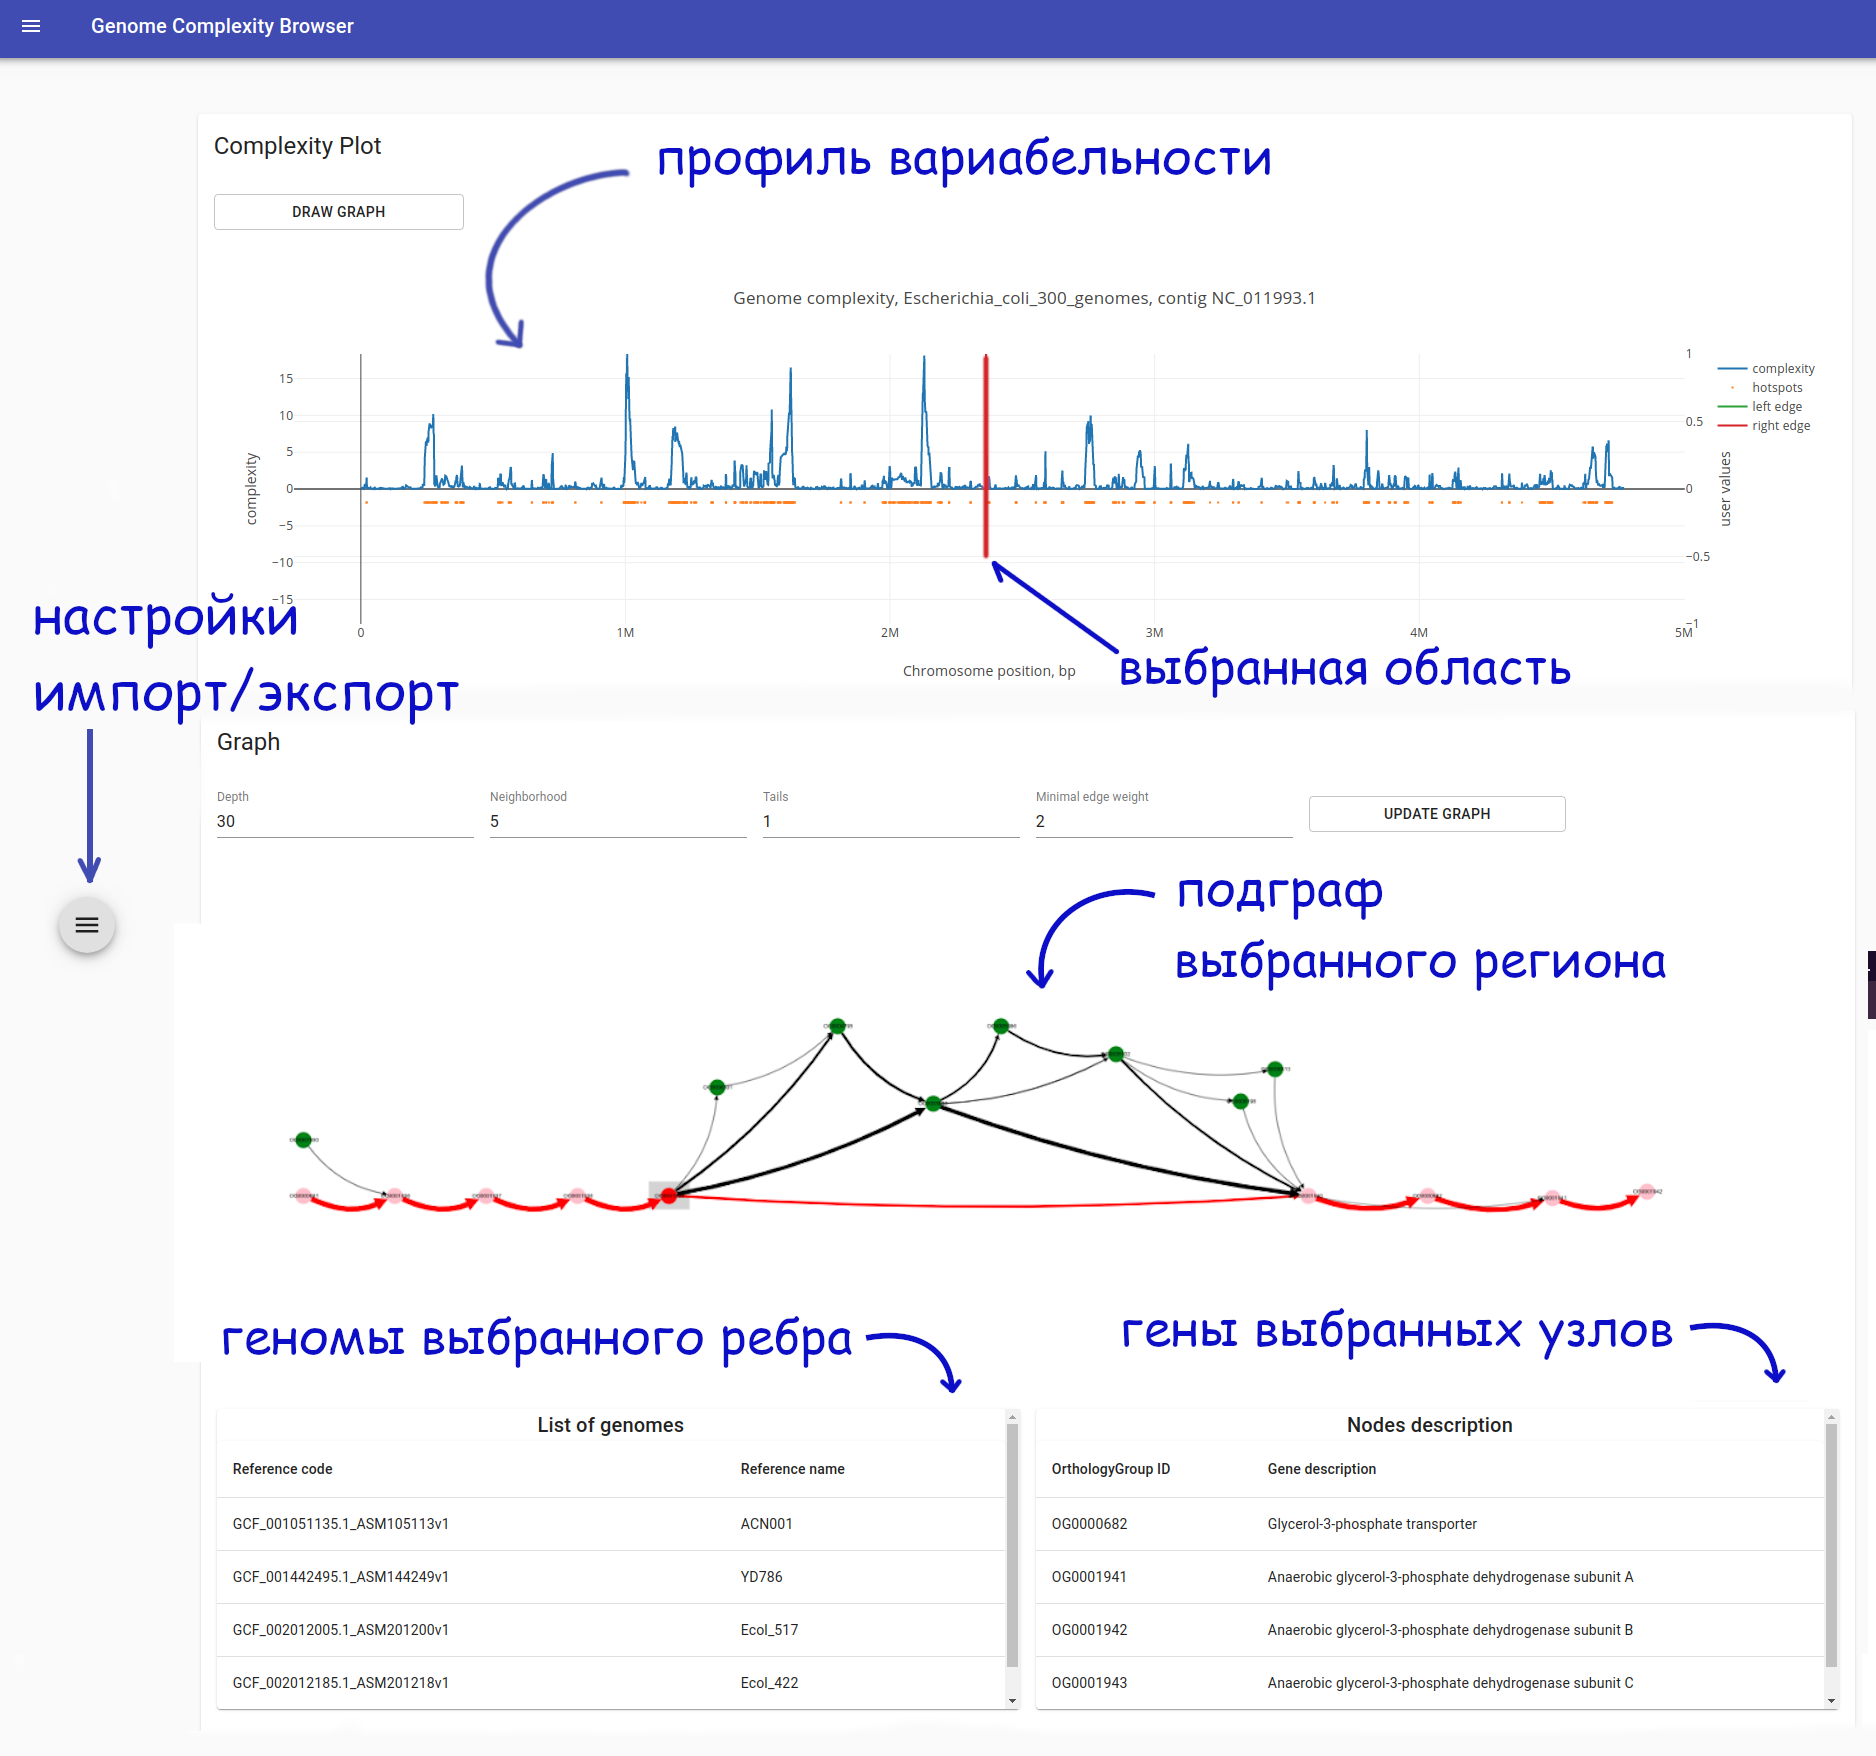
\includegraphics [width=0.9\textwidth] {Dissertation/images/gcb/gcb_face_text.png}
	\caption{Графический интерфейс программы Genome Complexity Browser.}
	\label{img:gcb_face}
\end{figure}

Основные сценарии использования программы следующие:

I. Интерес представляет некоторый оперон или группа генов.

Пользователь выбирает организм, геном и задает координаты области интереса. Происходит построение подграфа для выбранной области. При необходимости, пользователь меняет параметры визуализации (например, увеличивает минимальный отображаемый вес ребра для исключения редко встречающихся комбинаций генов, в случае если получаемый граф слишком сложен для анализа). Экспорт полученной визуализации в графическом формате, либо в формате XML для последующей визуализации подграфа в программе Cytoscape (графовый редактор). 

II. Интерес представляют области повышенной либо пониженной изменчивости генома.

Пользователь выбирает организм и геном. Происходит визуализация профиля изменчивости выбранного генома. Пользователь может выбрать интересующий его регион генома (например, область с максимальным уровнем изменчивости) и выполнить визуализацию подграфа в данной области - таким образом можно установить, какие гены содержатся в данном локусе у различных геномов, и каков паттерн зафиксированных в ходе эволюции изменений. Пользователь может экспортировать профиль изменчивости в виде текстового файла, для последующей визуализации (например, сравнение профилей изменчивости разных организмов), либо сохранить области с повышенной изменчивостью в файл в формате BED. 

\textbf{Возможности программы}

В программе предусмотрено автоматическое выделение "горячих точек"\ изменчивости. Они отображаются на профиле изменчивости (точки оранжевого цвета, расположенные ниже профиля), и их положение можно скачать в виде файла в формате BED. Для выделения областей повышенной изменчивости, мы использовали критерий Тьюки: искали значения уровня вариабельности, которые превышают 75 перцентиль на полтора межквартильных расстояния \cite{tukey1977exploratory}. 

Для анализа геномов, недоступных на веб-сервере \url{https://gcb.rcpcm.org}, необходимо использование локальной версии программы. Вначале подготовить (расположить в одной папке) интересующие пользователя геномы, затем запустить конвеер orthoSnake (доступен по адресу: \url{https://github.com/paraslonic/orthosnake}) и консольное приложение gg.py (доступно по адресу \url{https://github.com/DNKonanov/geneGraph}) - в итоге, будет создан файл с базой данных, содержащей графовое представление геномов и значения изменчивости. Файл с базой данных необходимо скопировать в папку, куда была установлена локальная версия сервера GCB, после этого можно работать с интерфейсом программы в веб-браузере. Схема анализа показана на рисунке~\ref{img:gcb_scheme}, полный пример (с установкой всех зависимостей и проведением анализа) доступен по адресу: \url{https://gcb.readthedocs.io/en/latest/standalone.html#complete-step-by-step-example}.

\begin{figure}[!ht] 
	\center
	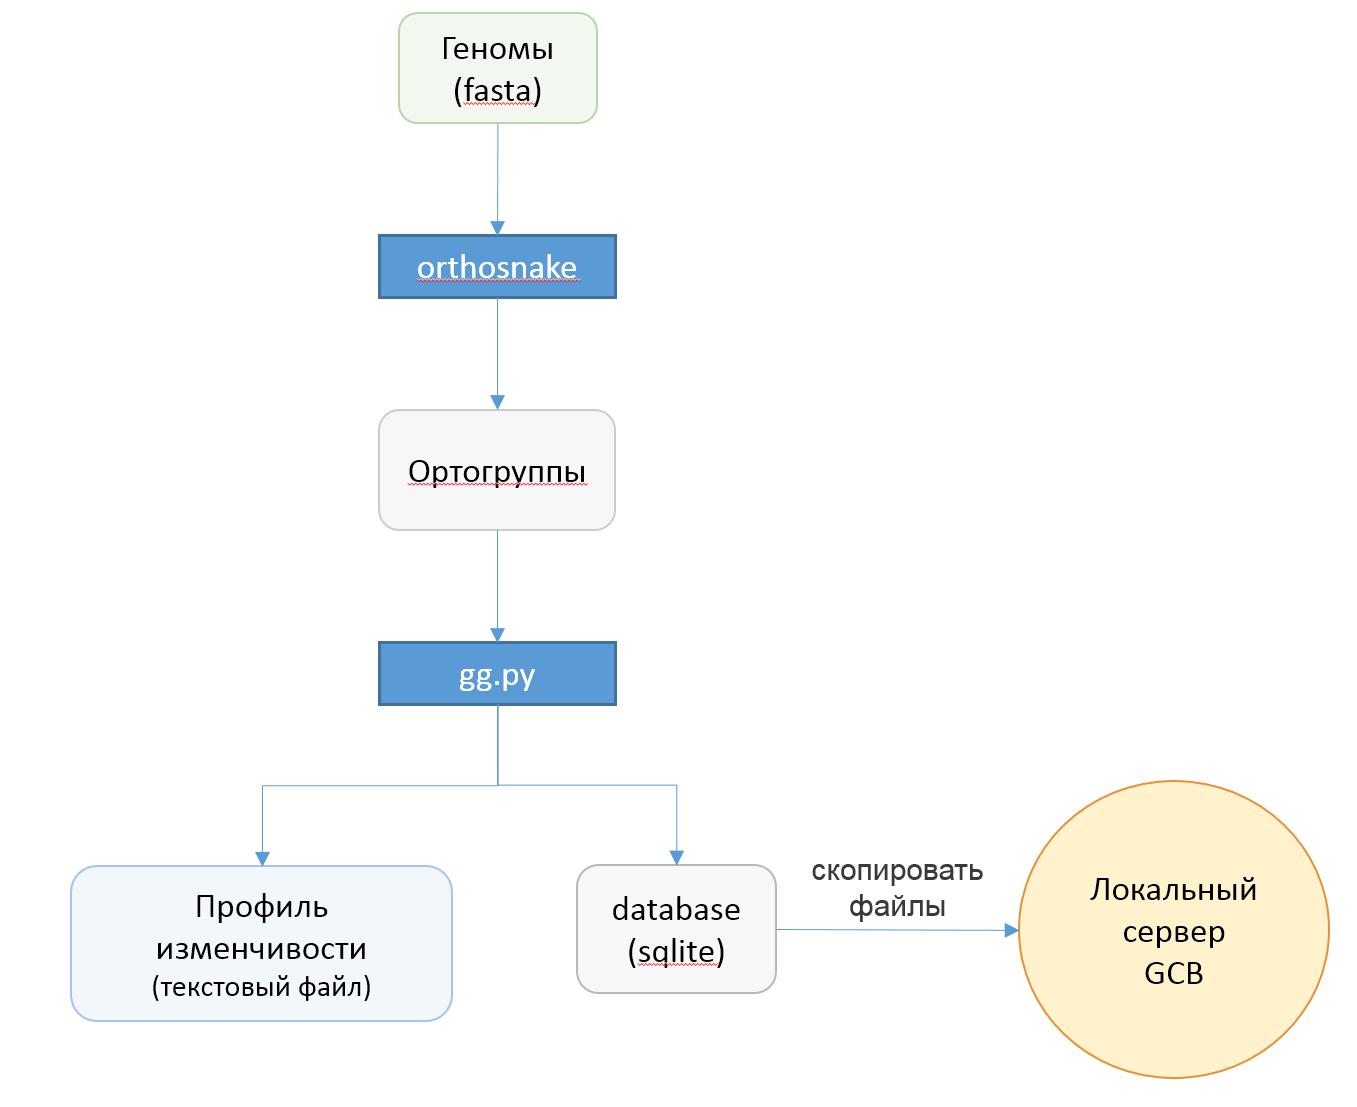
\includegraphics [width=0.9\textwidth] {Dissertation/images/gcb/standalone_scheme.png}
	\caption{Схема обработки геномных последовательностей при использовании Genome Complexity Browser на локальном компьютере.}
	\label{img:gcb_scheme}
\end{figure}

Документация и видеоматериалы по использованию программы (как веб-версии, так и консольных утилит) доступны по адресу \url{https://gcb.readthedocs.io}. 
